\chapter{在\glsentryname{java}里读写文字文件}

\begin{remark*}
    本章是用来测试排版的.
\end{remark*}

\begin{remark*}
    本章讨论的文件都是文字文件,
    而不是所谓的 ``二进制文件''.
\end{remark*}

\gls{java}是一门比较繁琐的电脑话.
所以, 在别的电脑话里简单的任务对\gls{java}而言不一定简单.
我姑且展现一下用相当基础的\gls{java}辛读或写文字文件会怎样罢.

首先, 我们需要一个包处理异常.
\begin{lstlisting}[language=Java]
import java.io.IOException;
\end{lstlisting}

\section{读文件}

读文件基本上算是比较容易的.
首先, 导入二个跟读文件相关的包.
\begin{lstlisting}[language=Java]
import java.io.BufferedReader;
import java.io.FileReader;
\end{lstlisting}

然后, 我们就可以施加魔法了.
\begin{lstlisting}[frame=single,language=Java]
public static String read(String txtFile,
        String fallback) {
    try (FileReader fr = new FileReader(txtFile);
            BufferedReader br = new BufferedReader(fr)) {
        StringBuffer sb = new StringBuffer();
        String s = null;
        while ((s = br.readLine()) != null) {
            sb.append(s).append("\n");
        }
        return sb.toString();
    } catch (IOException e) {
        return fallback;
    }
}
\end{lstlisting}

这里, 我姑且提一提 \lstinline[language=Java]`try` 后的圆括号.
在括号里, 我们可追加一些 ``需要被关闭的东西''
(具体地, 就是有 \lstinline[language=Java]`close()` 方法的对象),
它们可被自动地关闭.
曾经, 我们可能要这么写代码:
\begin{lstlisting}[frame=single,language=Java]
public static String read(String txtFile,
        String fallback) {
    FileReader fr = null;
    BufferedReader br = null;
    try {
        fr = new FileReader(txtFile);
        br = new BufferedReader(fr);
        StringBuffer sb = new StringBuffer();
        String s = null;
        while ((s = br.readLine()) != null) {
            sb.append(s).append("\n");
        }
        return sb.toString();
    } catch (IOException e) {
        return fallback;
    } finally {
        if (br != null) {
            try {
                br.close();
            } catch (IOException e) {
                e.printStackTrace();
            } finally {
                if (fr != null) {
                    try {
                        fr.close();
                    } catch (IOException e) {
                        e.printStackTrace();
                    }
                }
            }
        }
    }
}
\end{lstlisting}

可以看到, 为了避免资源泄露 (\gls{eng}: resource leak),
要写不少 \lstinline[language=Java]`try`.
这里, 我们还只是使用简单的
\lstinline[language=Java]`BufferedReader`
跟
\lstinline[language=Java]`FileReader`;
如果我们要实现更细致的需求,
那可能要关闭更多的资源,
从而要嵌套更多的代码.

\section{写文件}

写文件就稍复杂一些.
首先, 导入三个跟写文件相关的包.
\begin{lstlisting}[language=Java]
import java.io.BufferedWriter;
import java.io.File;
import java.io.FileReader;
\end{lstlisting}

我们暂且不考虑所谓的 ``权限''.
假如我们欲写入的文件已存在,
我们是想覆盖它,
还是想添加内容到文件末尾呢
(当然, 也会有其他的需求;
不过, 我们暂且不考虑它们)?
考虑到这二种模式很常用,
故在方法里加一个参数是个明智的选择.

\begin{lstlisting}[frame=single,language=Java]
public static boolean write(String txtFile,
        String str,
        boolean append) {
    File f = new File(txtFile);
    try {
        f.getParentFile().mkdirs();
        f.createNewFile();
    } catch (Exception e) {
        e.printStackTrace();
        return false;
    }
    try (FileWriter fw = new FileWriter(f, append);
            BufferedWriter bw = new BufferedWriter(fw)) {
        bw.write(str);
        return true;
    } catch (IOException e) {
        e.printStackTrace();
        return false;
    }
}
\end{lstlisting}

此处有一个小小的细节.
我使用了二个 \lstinline[language=Java]`try`:
前一个 \lstinline[language=Java]`try` 创建文件 (若其不存在),
而后一个 \lstinline[language=Java]`try` 向文件写入内容.

无妨假定我们想创建一个名为 \verb`./test/hi`
的文字文件 \lstinline[language=Java]`f`,
并向其写入 \verb`HI!`.
那么, \lstinline[language=Java]`f.getParentFile()`
就是 \verb`./test` 目录
(姑且称其为 \lstinline[language=Java]`g`).
假如 \lstinline[language=Java]`g` 存在,
那么 \lstinline[language=Java]`g.mkdirs()`
相当于不干任何事;
不过, 若其不存在, 则 \lstinline[language=Java]`g.mkdirs()`
可建立此目录.
类似地, 若文件 \lstinline[language=Java]`f` 已存在,
则 \lstinline[language=Java]`f.createNewFile()`
相当于不干任何事;
不过, 若其不存在,
则 \lstinline[language=Java]`f.createNewFile()`
可建立此文件.
值得注意的是, 若 \lstinline[language=Java]`g` 不存在,
则 \lstinline[language=Java]`f.createNewFile()`
是不可正常工作的.

若 \lstinline[language=Java]`f` 不存在,
则 \lstinline[language=Java]`new FileWriter(f, append)`
无法正常工作.
所以, 前一个 \lstinline[language=Java]`try` 是不可少的.

\section{添加一些细节}

我们可考虑封装读文件的方法与写文件的方法为一个类;
这样, 我们就可以方便地复用代码.
同时, 为了方便他人阅码, 我们最好加入一些注释.
这样, 我们就得到了如下代码.

% The "import" package does not seem to govern \lstinputlisting.
\lstinputlisting[
    frame=single,
    language=Java,
    caption={\lstinline`./listings/ReadAndWrite.java`},
    label={lst:ReadAndWrite}
]
{listings/ReadAndWrite.java}

最后, 我也要指出:
\begin{itemize}
    \item 我的实现不一定好;
          我的实现也不是很 ``简单'' (跟\gls{python}比).
    \item 我用的\gls{java}辛也比较老了.
          我也说过, 我一般用\gls{vsc}写文字文件 (当然包括代码).
          为了使\glssymbol{vsc}提供的%
          \emph{\gls{java}话插件}工作,
          我得使用\gls{java}~11 或更高版本的\gls{java}.
          可是, 我在桌面环境里安装了桌面宠物 (图~\ref{fig:Girls}),
          而这需要较低版本的\gls{java}才可正常地工作.
          所以, 我的解决办法也很简单:
          ``安装'' \gls{java}辛,
          且为\glssymbol{vsc}单独准备一个
          ``免安装版'' \gls{java}~17.
    \item 应该不会有人想从本章学写\gls{java}罢?
    \item 应该不会有人想从本书学\gls{math}罢 (确信).
\end{itemize}

\begin{figure}[h!]
    \centering
    \begin{minipage}{0.3\textwidth}
        
\includegraphics[width=\textwidth]{Rei}
        \subcaption{レイ}
    \end{minipage}
    \hspace{0.15\textwidth}
    \begin{minipage}{0.3\textwidth}
        
\includegraphics[width=\textwidth]{Ruka}
        \subcaption{ルカ}
    \end{minipage}
    \caption{Two \textit{Kotonoha Amrilato} characters}
\end{figure}

\begin{figure}[h!]
    \centering
    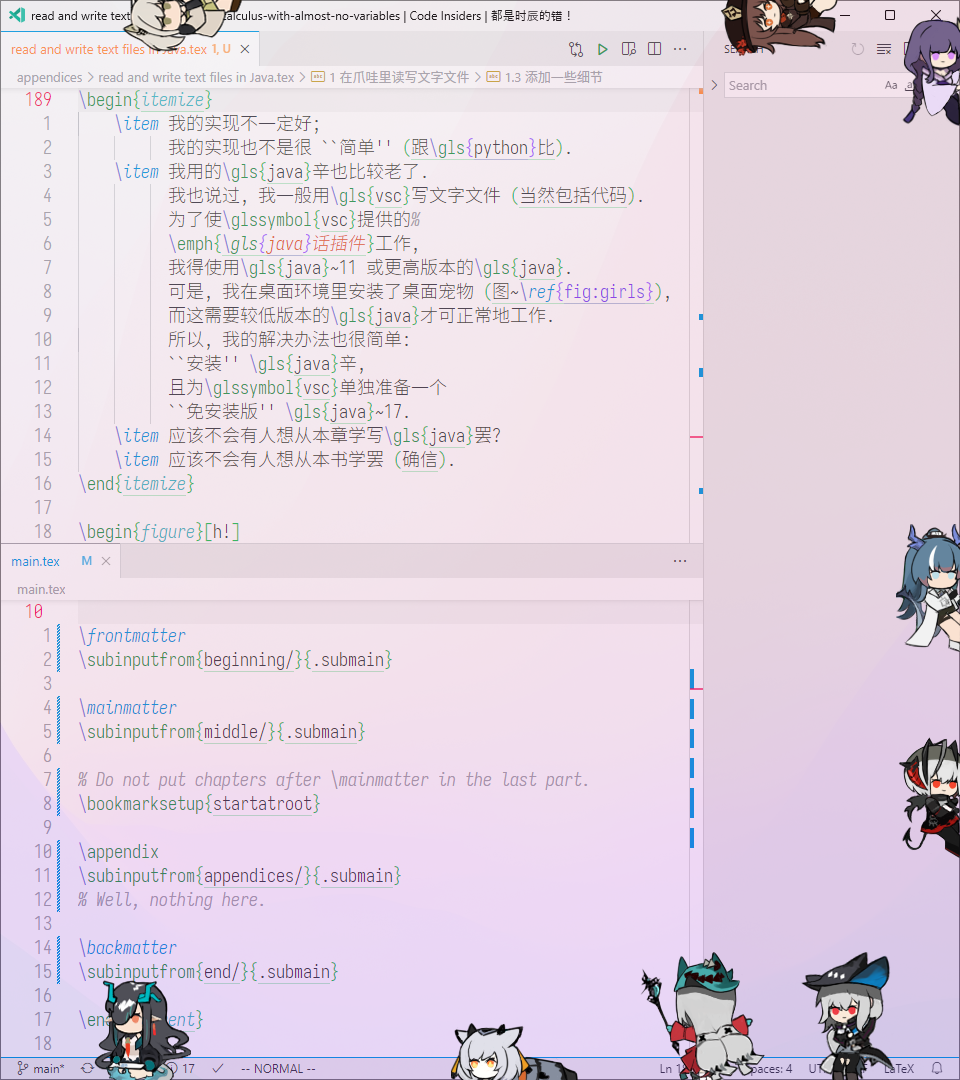
\includegraphics[width=\textwidth]{girls}
    \caption{桌面宠物}
    \label{fig:Girls}
\end{figure}

\section{后续}

\begin{remark*}
    本节算是所谓的支线故事罢.
\end{remark*}

我于 2022~年 5~月 22~日在哔哩哔哩上发了一个%
\href{https://www.bilibili.com/video/BV1JY4y157BX}{视频}.
它没有什么营养;
它就是以每 2~秒翻 2~页的速率展现了本书的正文.

我如何实现此事呢?
首先, 我打开书.
然后, 我翻到此书的页~1.
接着, 我还是用\gls{java}写了个机器人帮我翻页.
当然了, 我肯定还开了屏幕录制.
最后, 我也不必修改录制的结果, 直接上传它到哔哩哔哩.

\lstinputlisting[
    frame=single,
    language=Java,
    caption={\lstinline`./listings/KeyPress.java`},
    label={lst:KeyPress}
]
{listings/KeyPress.java}

我用到了 \verb`Robot` 类.
它的功能还是很强大的.
我认为,
\verb`keyPress()` 跟 \verb`keyRelease()`
是二个关键的方法.
\verb`KeyEvent` 类使我方便地召唤一个键.
假如没有它,
我就要手动输入 ``右键'' 的编码了.
当然了, \verb`delay()` 也很好用.
毕竟, 我要给观众 2~秒读 2~页书.
\verb`2000` 就是 \num{2000}~毫秒.
前面的 \verb`delay(20000)` 相当于给我
20~秒的准备时间.
利用循环, 我就可以反复地按一个键, 并松开之.

我姑且称码~\ref{lst:KeyPress} 的风格为
``\gls{python}\gls{java}'' 罢.
我是融合怪罢.

好的.
我姑且说到这里罢.
